%!TEX root = ../ENTRUST_TR.tex
%This section will explain how we achieved our goal.
To illustrate how \approach\ is capable of assuring runtime compliance of a self-adaptive system with its non-functional Quality-of-Service (QoS) requirements,  we developed a simulator for the  unmanned underwater vehicle (UUV) embedded system (Section~\ref{sec:example}), using the open-source framework MOOS-IvP\footnote{\url{http://oceanai.mit.edu/moos-ivp}}. Note that  in \approach\ self-adaptive systems there is separation of concerns between the managed system (i.e., the UUV and how it works) and the managing system (i.e., the autonomic component that enables a system to adapt). This consideration is in line with the autonomic computing vision~\cite{Kephart2003:Comp}. In this realisation of \approach, the focus is on the managing element; we omit any details about how the actual  UUV operates. In the following paragraphs, we explain how we use \approach\ to provide offline and online assurances for the UUV self-adaptive system.

\subsection{Online assurances}
The managing system adopts the MAPE-K (Monitor--Analyse--Plan--Execute--Knowledge) autonomic control loop proposed by Kephart and Chess~\cite{Kephart2003:Comp}. Also, the managing system uses probes and effectors to receive input from and send instructions to the managed system, respectively. In the following paragraphs we describe briefly the automata we developed for realising \approach\ in the UUV embedded system.

\subsubsection{Monitor.}
Monitor automaton receives sensors rates from probes. After that, the monitor automaton checks whether the received sensor rates are equal to the previously measured sensor rates. If both rates are equal, there is no need for adaptation; hence \approach\ terminates and does not continue with the remaining MAPE-K control loop steps. If the sensor rates are different, then analysis is required and the monitor automaton invokes the analyse automaton sending a \textit{start\_analysis!} signal as shown in Figure~\ref{fig:monitor-automaton}. 

\begin{figure}[h!]
	\centering
	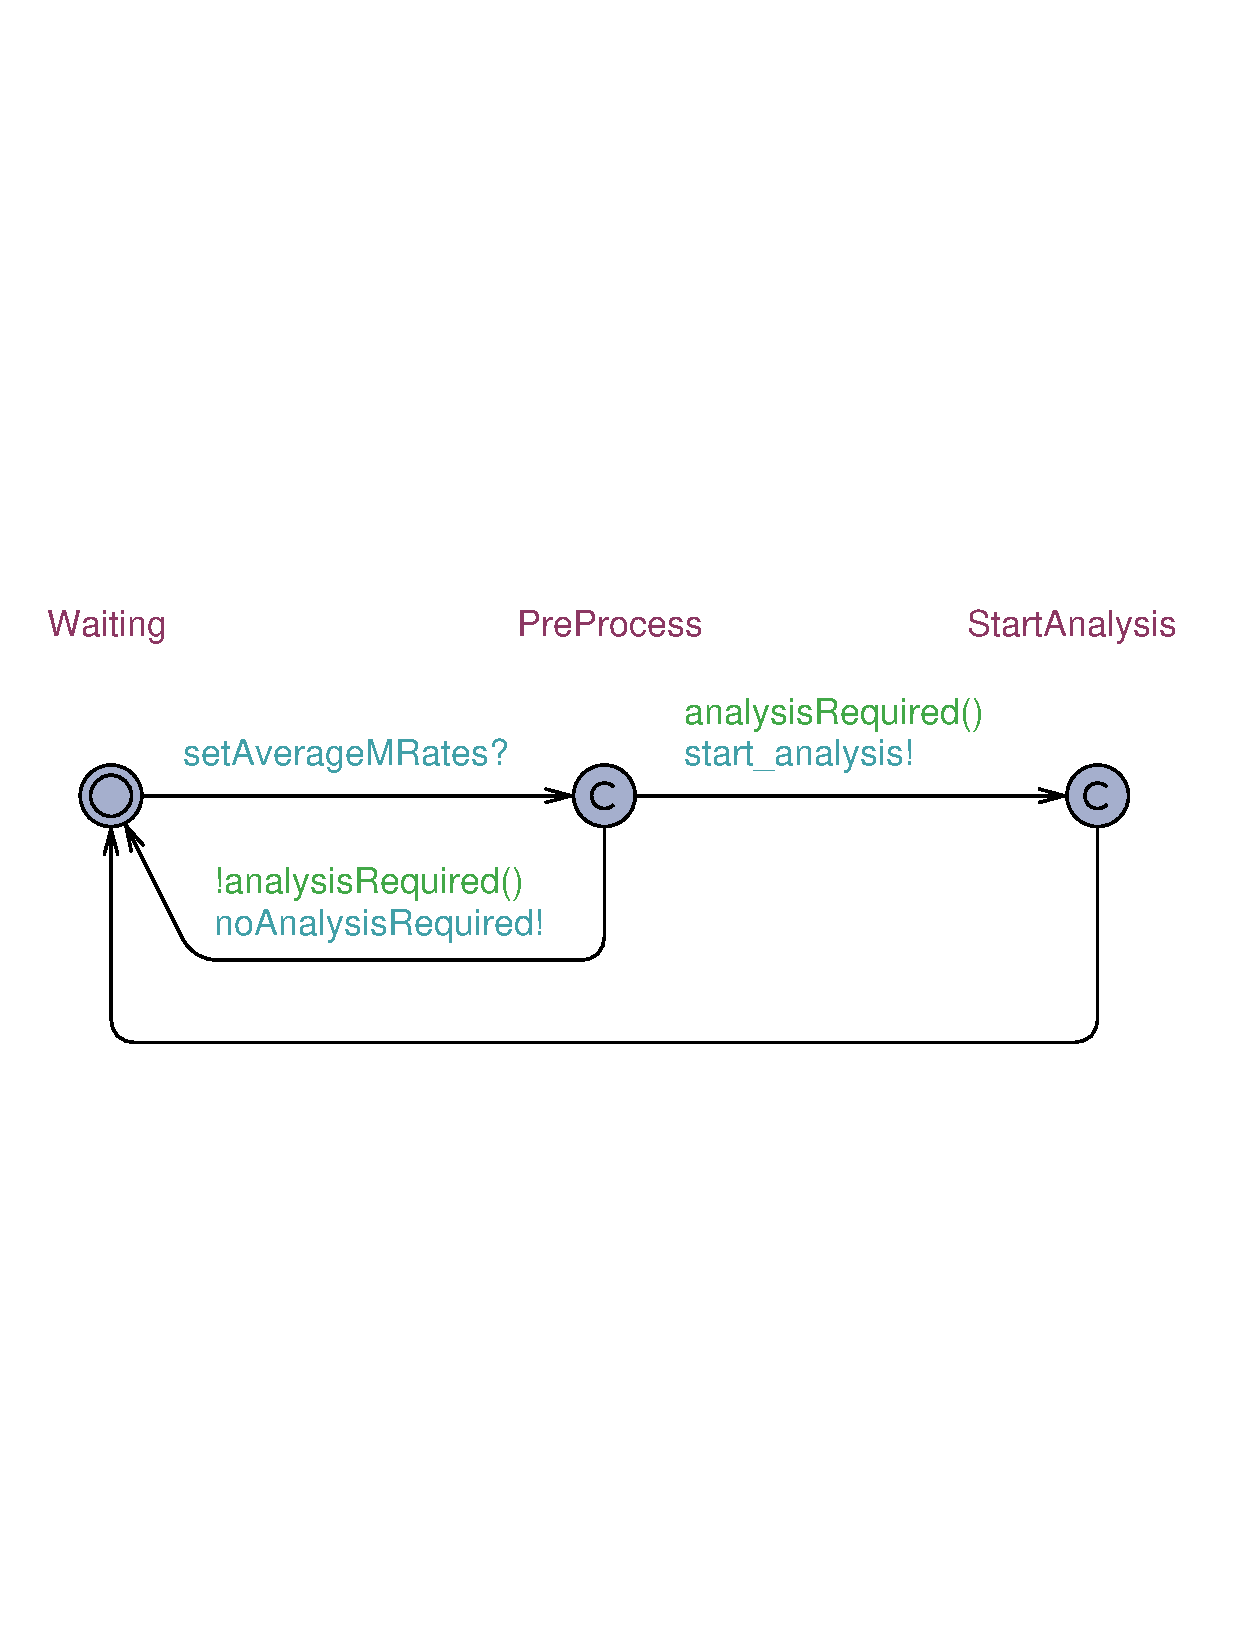
\includegraphics[trim = 10mm 100mm 0mm 125mm, clip, width=0.5\linewidth]{figures/Monitor.pdf}
	\caption{Monitor automaton of our UUV embedded system}\label{fig:monitor-automaton}
	
	\vspace*{-2mm}
\end{figure}

\subsubsection{Analyser.}

\begin{figure}[b]
	\centering
	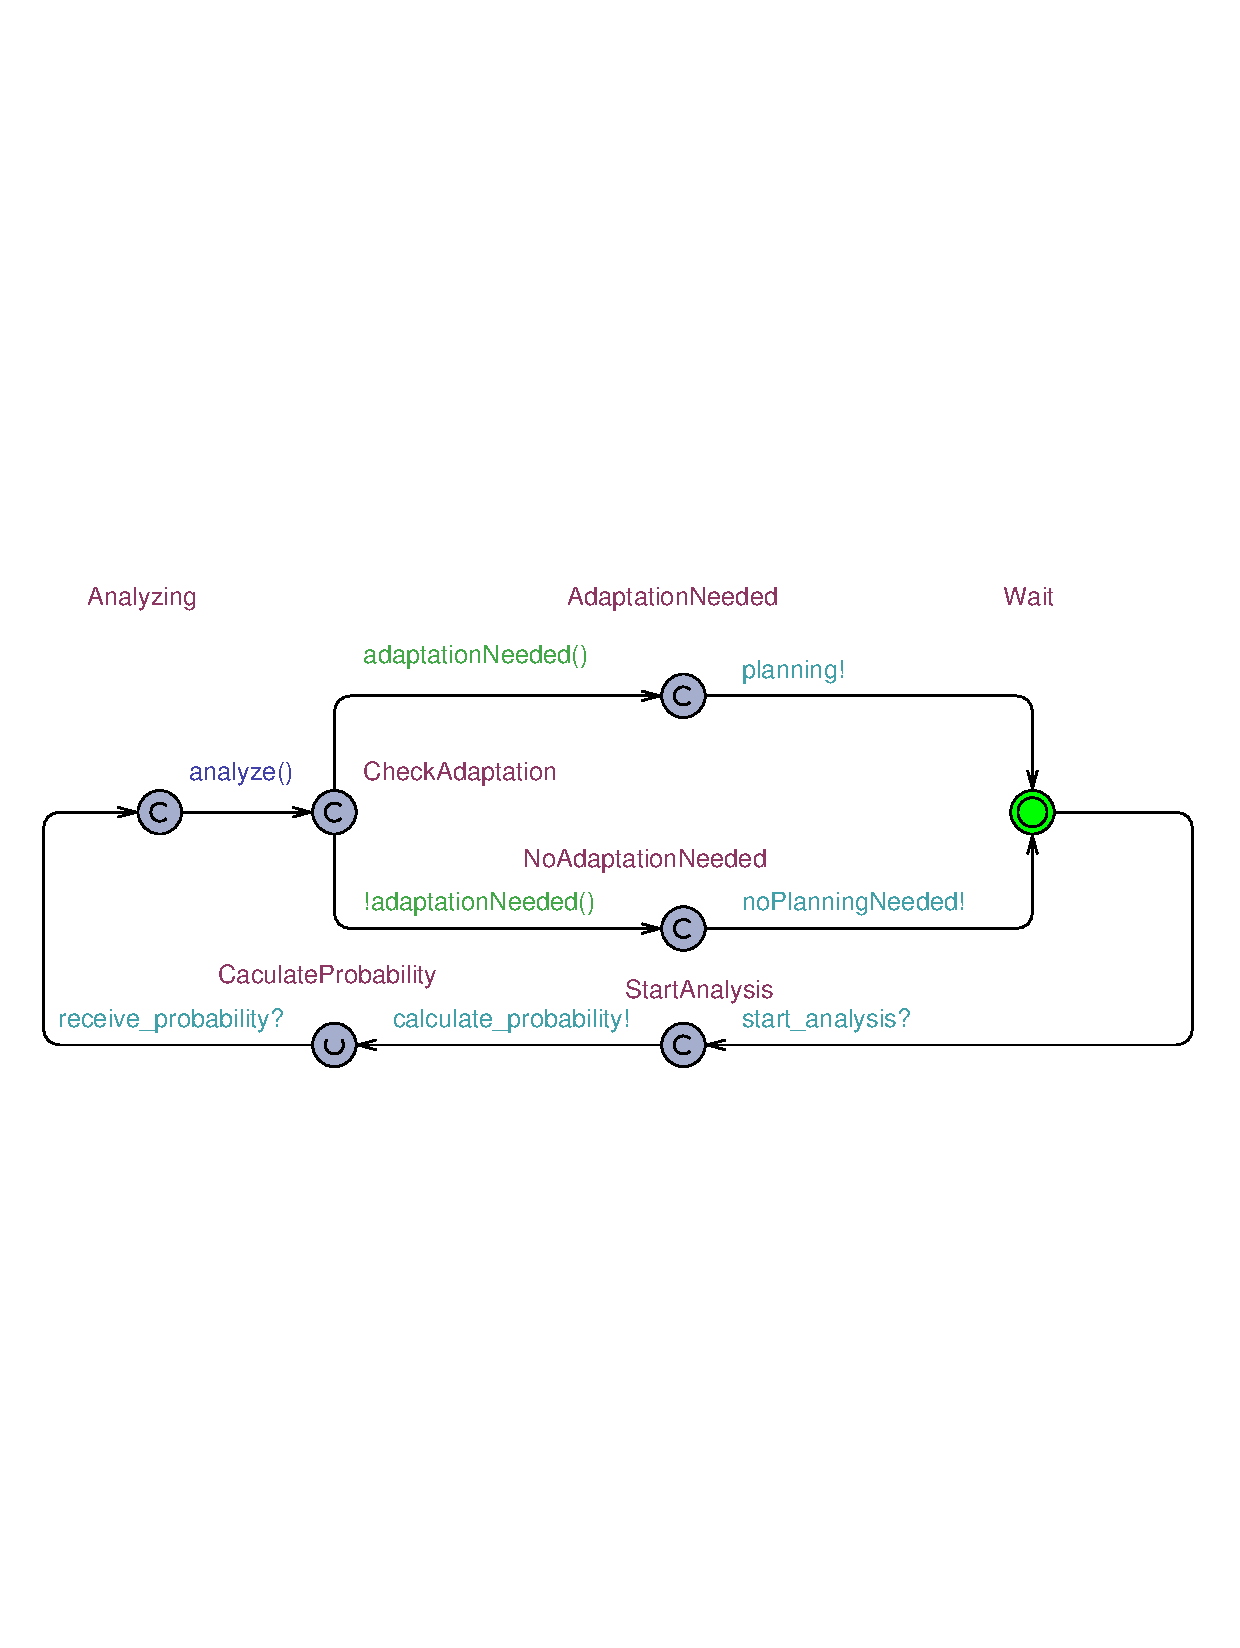
\includegraphics[trim = 5mm 95mm 0mm 105mm, clip, width=0.8\textwidth]{figures/Analyzer}
	\caption{Analyze automaton of our UUV embedded system}\label{fig:analysis-automaton}
	
	\vspace*{-2mm}
\end{figure}

Analyse automaton takes the current measured rates of sensors and tries to find the best configuration which satisfies requirements R1, R2 and R3. Figure~\ref{fig:analysis-automaton} depicts the analyse automaton. The automaton starts the analysis as soon as it receives the signal \textit{start\_analysis?} from the monitor automaton. It then
sends the signal \textit{calcProbability} along with the sensor rates and invokes RQV to carry out quantitative analysis. For this operation we use an embedded instance of the probabilistic model checker PRISM~\cite{Kwiatkowska2011:CAV}. This analysis evaluates all the possible system configurations for the current environment state (i.e., rates of sensors). The analyse automaton receives the quantitative verification results through the \textit{recvProbability?} channel. Next, it examines the received set of configurations and determines the configuration that satisfies requirements R1 and R2, and optimises requirement R3. Once the best configuration is found, the automaton compares the new configuration to the current best configuration. If the configurations are the same, there is no need to proceed to planning. If adaptation is required, the analyse automaton invokes the planner sending the signal~\textit{planning!}.


\subsubsection{Planner.}
The plan automaton is responsible for establishing an adaptation policy. It starts running when the signal ~\textit{planning?} is received. First, it  creates the plan steps for the new configuration of sensors, i.e., whether a sensor should be turned on or off. To this end, the plan automaton checks the current sensor configuration with the new configuration and determines whether there is a need to make a change to one or more sensors. If the current sensor configuration is same as in the new configuration, there is no need to create a plan step. Otherwise, if the sensor configurations do not match, then the plan automaton creates the plan step, according to the new configuration. When all sensors are checked, the plan automaton checks  if the current UUV speed is different to the new UUV speed and if this true, it creates a new plan step to change the speed of the UUV. Finally, the plan automaton invokes the execute automaton by sending the~\textit{execute!} signal. Figure~\ref{fig:plan-automaton} shows the plan automaton of the UUV.

\begin{figure}[h!]
	\centering
	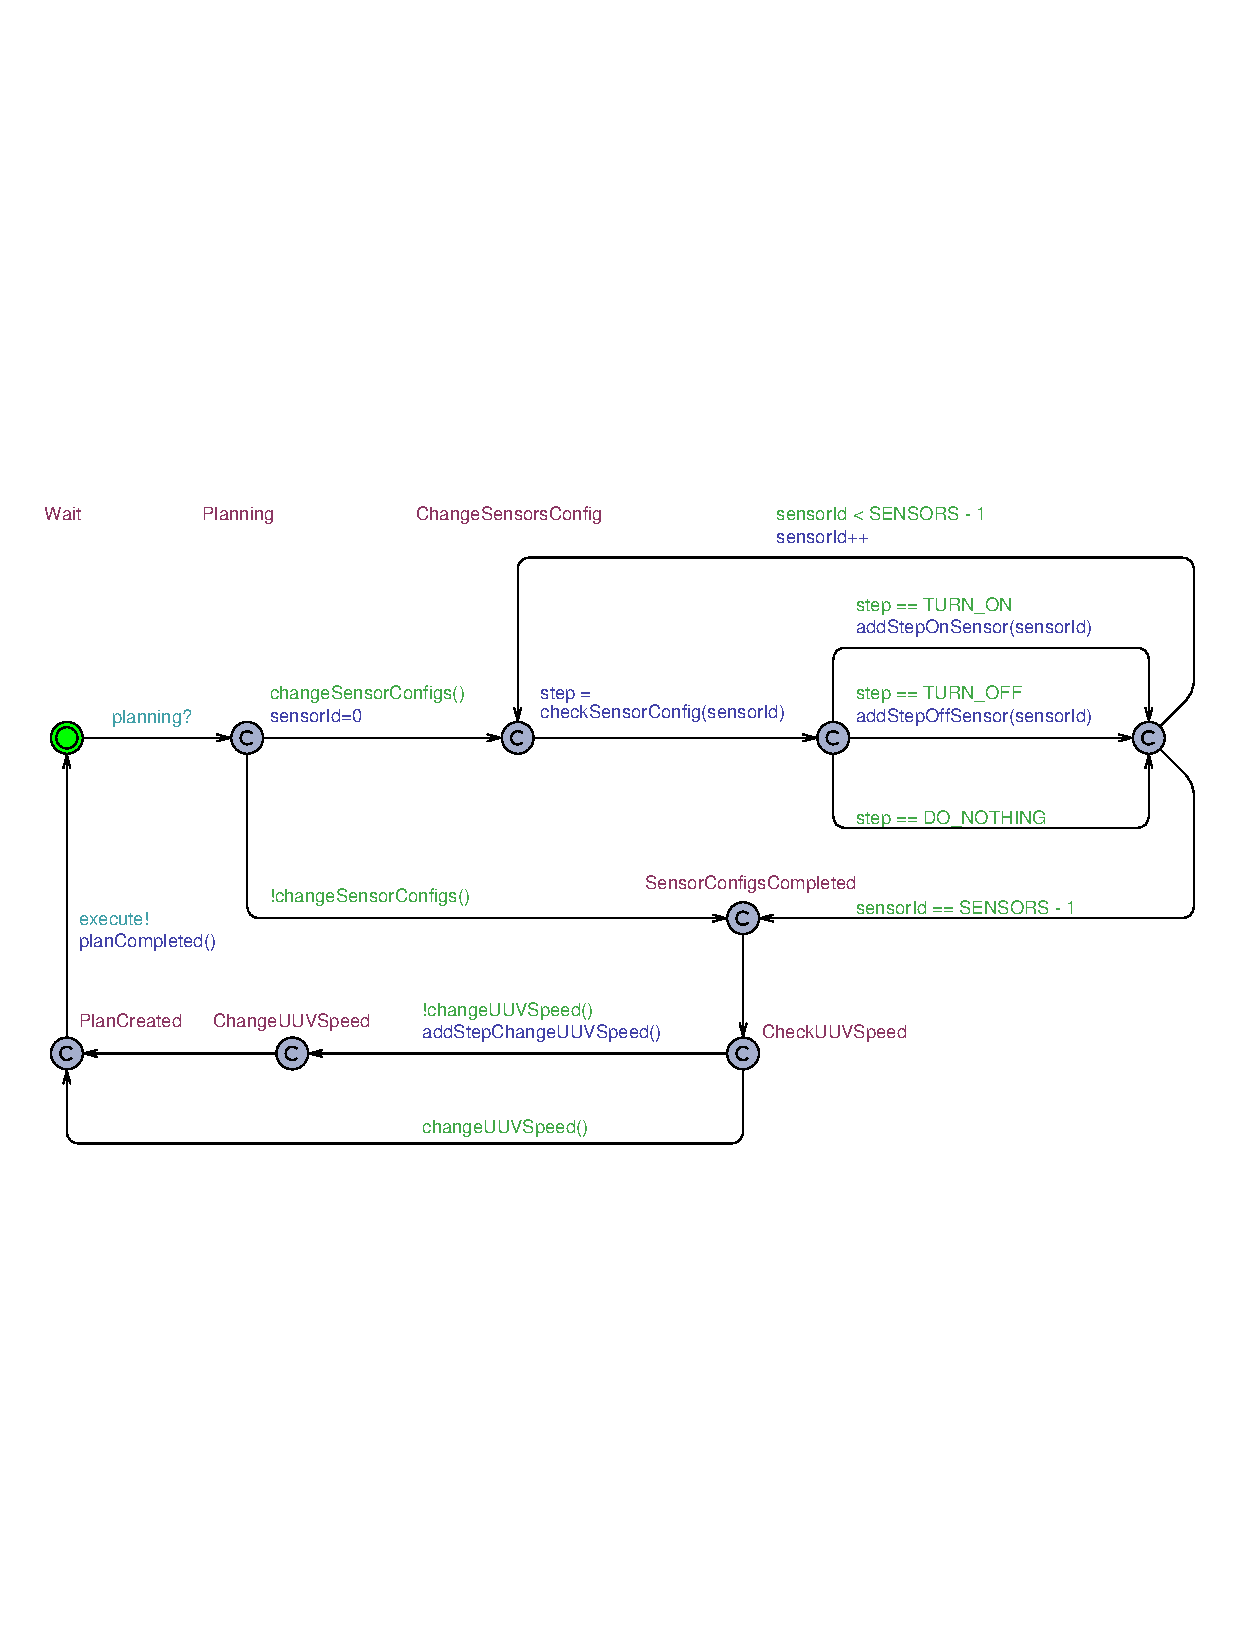
\includegraphics[trim = 5mm 80mm 0mm 90mm, clip, width=\linewidth]{figures/Planner.pdf}
	\caption{Plan automaton of our UUV embedded system}\label{fig:plan-automaton}
	
	\vspace*{-2mm}
\end{figure}


\subsubsection{Executor}
The execute automaton starts after receiving the signal~\textit{execute?} from the plan automaton. It then goes through all the plan steps, one-by-one, and executes them. The operation completes when the signal~\textit{allPlanStepsExecuted!} is sent. The plan automaton is presented in the Figure~\ref{fig:execute-automaton}.

\begin{figure}[t]
	\centering
	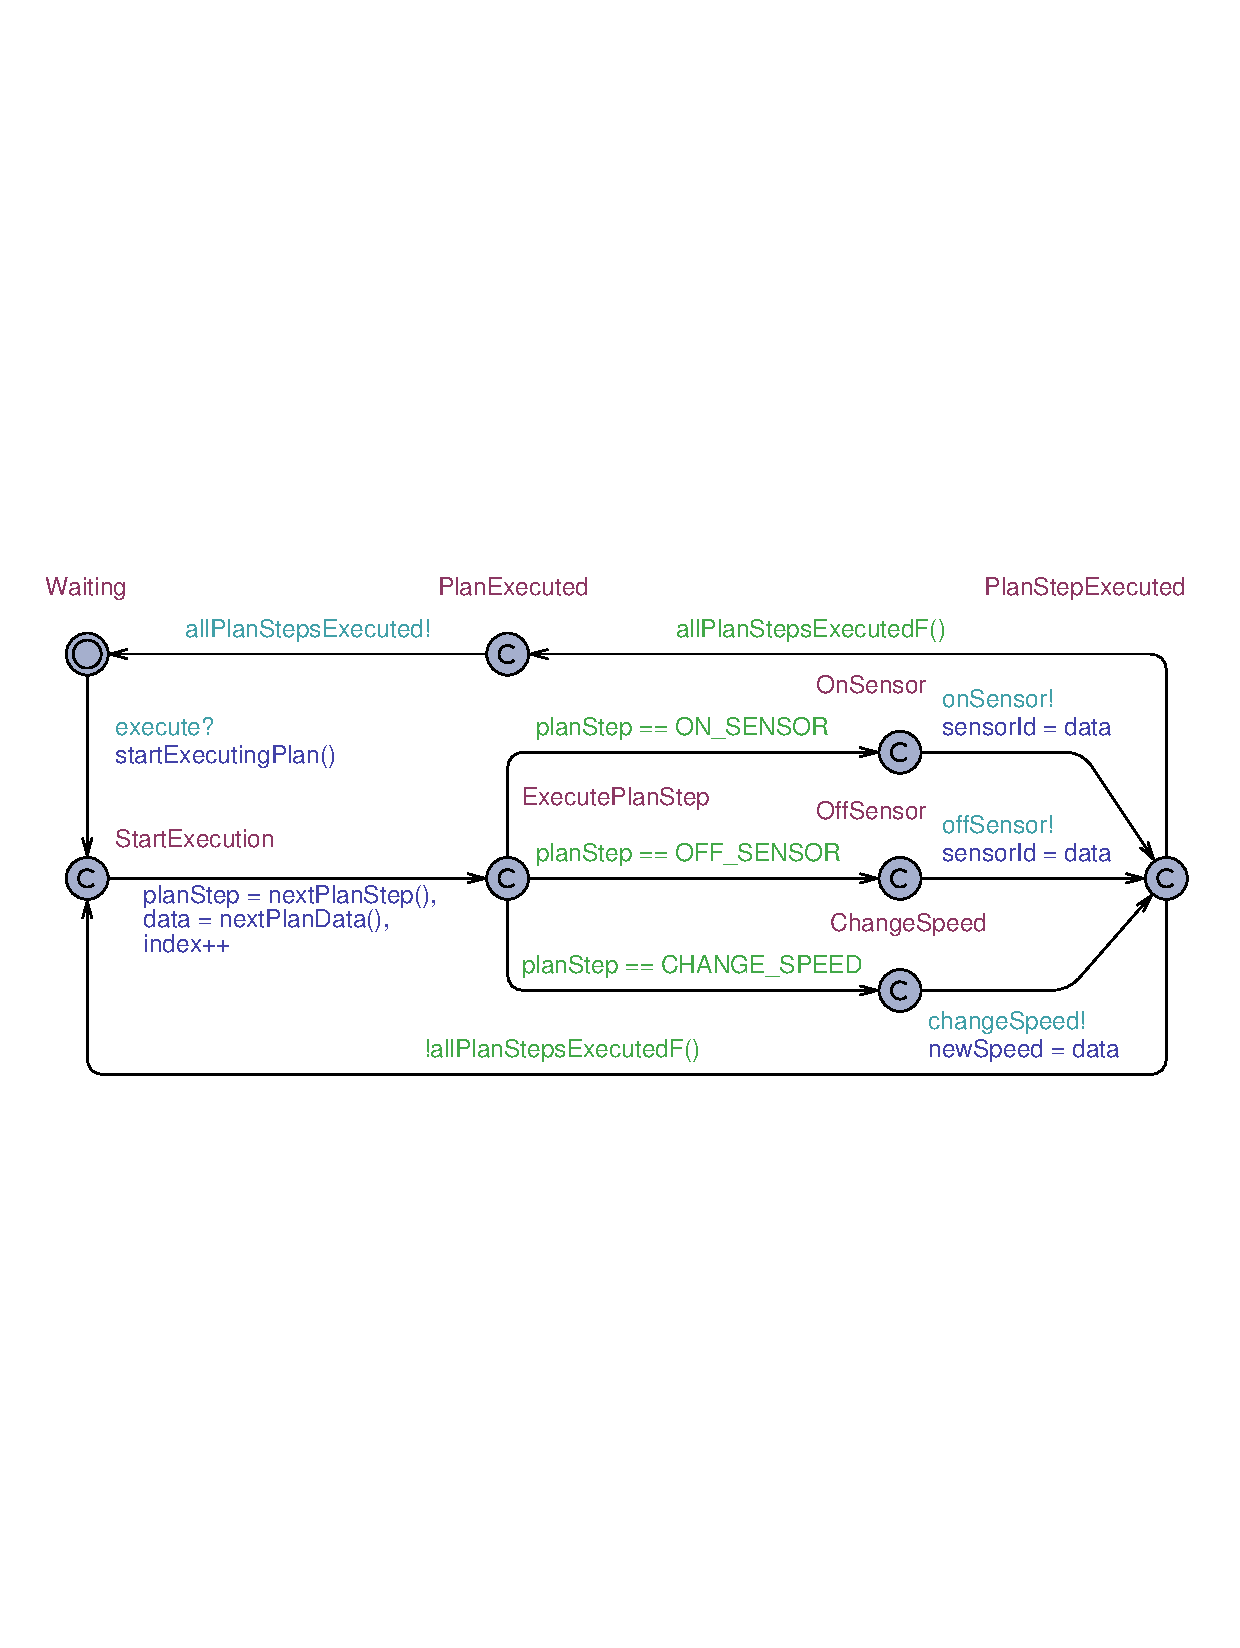
\includegraphics[trim = 10mm 95mm 5mm 105mm, clip, width=\textwidth]{figures/Executor}
	\caption{Execute automaton}\label{fig:execute-automaton}
	
	\vspace*{-2mm}
\end{figure}


%\subsection{Probes \& Effectors}
%If necessary code of probes \& effectors

\subsection{Offline Assurances}
We used \approach\ to produce offline assurance evidence for the UUV embedded self-managing system. We verified both the MAPE-K autonomic control loop and the QoS system requirements (Section~\ref{sec:example}) using the knowledge part which comprises the probabilistic and automata models. For the verification of the MAPE-K control loop we checked various properties of the MAPE-K loop, e.g., if it is deadlock free and if its elements communicate and synchronise through signals. We also confirmed that each stage of this control loop operates as expected, e.g., if the analyser determines that no adaptation is required then it has to be the case that the current configuration is the same as the new configuration, if the planner creates an adaptation policy then the executor will realise this policy. For the verification of the QoS requirements, we used the nominal sensor rates (as defined in their specifications) and carried out the analysis stage to confirm that there is at least one policy satisfying the QoS requirements of the self-adaptive UUV system. In particular, we provided evidence for the compliance of the UUV system with requirements R1 and R2 (Section~\ref{sec:example}) verifying the following properties:
\begin{align*}
	A[] \textrm{current\_Configuration.R1\_Result} > 20 \ \\
	A[] \textrm{current\_Configuration.R2\_Result} < 120 
\end{align*}


%\subsection{Online Assurances}
%The perpetual provision of assurances online. How we are using both technologies together.